\section{Introducci�n}
\subsection{�Qu� es esto del \LaTeX?}

\begin{frame}[t]{Un procesador de textos: Del \TeX{} al \LaTeX{}}%[plain] para que ocupe toda la pantalla
\begin{block}{El \TeX{}}
\begin{itemize}
\item \pause Creado por Donald E. Knuth (Univ. de Stanford)
\item \pause Proviene de la palabra {\em technology}, cuya ra�z griega es $\tau\epsilon\chi\equiv$ {\em arte}
\item \pause Como todo lenguaje de programaci�n:
\begin{itemize}
\item Gran {\color{miverdeO}potencia} y {\color{miverdeO}flexibilidad}
\item {\color{red}Complejidad} para aquellos no familiarizados con la programaci�n
\end{itemize}
\end{itemize}
\end{block}

\begin{block}{El \LaTeX}
\begin{itemize}
\item \pause Leslie Lamport ({\em Digital Equipment Corp.})
\item \pause Conjunto de {\bf �rdenes} que acercan el \TeX{} a los mortales
\item \pause Se normaliza el \LaTeX{}: \LaTeX$2_\varepsilon$
\end{itemize}
\end{block}
\end{frame}

\subsection{�Por qu� utilizarlo?}

\begin{frame}{�Por qu� utilizarlo?}
\begin{multicols}{2}
\begin{itemize}
\item \pause Es software libre
\item \pause Funciona sobre casi cualquier tipo de sistema y arquitectura (incluso las gratuitas)
\item \pause {\color{red}Auto}enumera las f�rmulas y ecuaciones
\item \pause Crea �ndices de contenido, tablas, figuras y de t�rminos �{\color{red}auto}m�ticamente!
\item \pause Permite el uso de Bib\TeX{}
\item \pause Resultado profesional
\item \pause Buen soporte para las matem�ticas
\item \pause Para que las cosas queden monas ya est�n otros: {\color{red}\LaTeX{} lo hace por t�}
\item \pause Los archivos ocupan muy poco
\end{itemize}
\end{multicols}
\end{frame}

\begin{frame}{Dos filosof�as a la hora de procesar documentos}
\begin{columns}
\column{0.5\textwidth}
\pause\begin{defi}{WYSIWYG}
Acr�nimo de {\em What You See Is What You Get}
\end{defi}
\begin{ejem}{WYSIWYG}
\begin{itemize}
\item Word
\item Google Docs 
\item Wordpress
\item Open Office 
\item \ldots
\end{itemize}
\end{ejem}
\column{0.51\textwidth}
\pause\begin{defi}{WYSIWYM}
Acr�nimo de {\em What You See Is What You Mean}
\end{defi}
\begin{ejem}{WYSIWYM}
\vspace{0.8cm}
\centering
\invisible<1-3>{\Huge�\LaTeX{}!}
\pause\vspace{0.8cm}
\end{ejem}
\vfill
\end{columns}
\end{frame}

\subsection{�Merece la pena?}
\begin{frame}{Los inconvenientes\ldots �son inconvenientes?}
\begin{columns}[T]
\column[T]{0.7\textwidth}
\vspace{-2.5cm}
\uncover<1->{Los inconvenientes que la gente suele remarcar son:}
\begin{itemize}
\item <2->\alert<6>{\em ``Me frustra mucho la complejidad, �por qu� hacerlo tan dif�cil?''.}
\item <3->\alert<7>{\em  ``Tardo mucho en escribir un simple art�culo.''.}
\item <4->\alert<8>{\em ``Esto tambi�n lo hace Word''.}
\end{itemize}

\uncover<5->{Preg�ntate:}
\begin{itemize}
\item <6-> \alert<6>{�Cu�ntas palabras sabes entre el castellano y el ingl�s? �Qu� suponen algunas decenas m�s?}
\item <7-> \alert<7>{ �Cu�nto tardar�as en escribir algo en Word con la misma calidad?}
\item <8-> \alert<8>{�No est�s harto de coger el rat�n para insertar las f�rmulas? �No te gustar�a que los �ndices y las referencias se hicieran solos,  y los elementos flotantes no se comieran el texto?}
\end{itemize}
\column[c]{0.3\textwidth}
\vspace{0.5cm}

\begin{figure}
\centering
\begin{tikzpicture}
\alt<6->{\node[opacity=1]{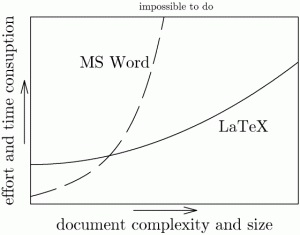
\includegraphics[width=\textwidth]{Figuras/CurvaAprendizaje2.jpg}};}
{\node[opacity=0.01]{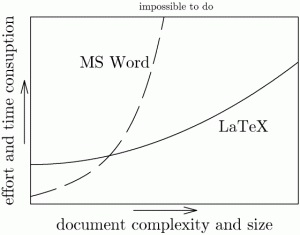
\includegraphics[width=\textwidth]{Figuras/CurvaAprendizaje2.jpg}};}
\end{tikzpicture}
\vspace{-0.75cm}
\uncover<6->{\caption{Coste {\em vs.} complejidad para \LaTeX{} y Word}}
\label{fig:CurvaAprendizaje}
\end{figure}
\end{columns}
\end{frame}

\subsection*{�nimo}